%----------------------------------------------------------
% PACKAGES AND THEMES
%----------------------------------------------------------
\documentclass[aspectratio=169,xcolor=dvipsnames,handout]{beamer}

\usetheme{Darmstadt}
\usecolortheme{seahorse}
\setbeamercovered{transparent}

\usepackage[hangul]{kotex}
\usepackage{hyperref}
\usepackage{graphicx, array, adjustbox, makecell}
\usepackage{booktabs, multicol, multirow}

% font조정
%\usepackage{fontspec}
%\setmainfont{Times New Roman}
%\setmainhangulfont{NanumGothic}

% 문자열 대체{노사관계론 전용}
\usepackage{newunicodechar}
\newunicodechar{•}{$\cdot$}
\newunicodechar{➔}{$\implies$}
\newunicodechar{∴}{$\therefore$}
\newunicodechar{∵}{$\because$}

%----------------------------------------------------------
% TITLE PAGE
%----------------------------------------------------------
\title{임금제도와 성과참가}
\subtitle{노사관계의 이론과 실제}
\author{오성재}
\institute[CNU]
{\relax
    충남대학교 경제학과\
    }
\date{2024년 10월 28일}

%----------------------------------------------------------
\begin{document}
%----------------------------------------------------------

\frame{\titlepage}

\begin{frame}{목차}
    \small
    \tableofcontents[hideallsubsections]
\end{frame}

\section{임금제도}
\subsection{임금제도의 개념}

\begin{frame}[allowframebreaks]
    \frametitle{임금제도의 의의와 중요성}
    \begin{block}{임금}
        사용자가 근로의 대상으로 근로자에게 지급하는 일체의 금품
    \end{block}
    \begin{itemize}[<+->]
        \item 기업측 중요성
        \begin{itemize}[<+->]
            \item 조직의 목표달성에 핵심적 요소인 생산성에 영향 합리적 임금설계 필수
            \item 상품의 제조원가의 상당부분 차지 해당 상품의 경쟁력 결정요소
            \item 노동시장에서 인력을 확보하는데 중요한 역할
        \end{itemize}
        \framebreak%
        \item 종업원측 중요성
        \begin{itemize}[<+->]
            \item 임금은 소득의 주 원천: 생리적 욕구 충족 및 생활의 질 향상에 중요한 역할
            \item 종업원의 사회적 지위 결정
            \item 사내에서 공식 직제상의 서열, 직무수행능력 및 성과에 따라 개인의 임금 결정. $\because$ 임금수준 자체가 종업원 직위의 판단기준
            \item 사회적으로 임금수준은 능력 있는 사람의 평가 잣대 역할
            \item 물질적으로 풍요로운 생활 영위
        \end{itemize}
    \end{itemize}
\end{frame}

\begin{frame}[allowframebreaks]
    \frametitle{임금관리의 목적}
    \begin{itemize}[<+->]
        \item 효율성: 임금의 수준에 있어서 직원간에 격차를 두어 직원의 동기유발을 위하여 공헌해야 함
        \item 공정성: 비슷한 자격 또는 동일한 공헌을 한 직원에게는 비슷한 수준의 임금을 지급하며 임금이 직원간 불만족의 원인이 되지 아니하게 함
        \item 적법성: 대부분의 국가에서 임금에 대한 많은 법령을 두고 이를 준수하여야 함
    \end{itemize}
\end{frame}

\subsection{임금의 여러 개념}%

\begin{frame}[allowframebreaks]
    \frametitle{임금수준의 관리}
    \begin{block}{임금수준 (pay level)}
        기업이 모든 구성원들에 대해 지불하는 임금률의 평균으로 일반적으로 기업전체의 임금수준, 즉 일정한 기간에 한 기업 내의 모든 종업원에게 지급되는 평균임금
    \end{block}
    \begin{enumerate}[<+->]
        \item 생계비: 임금은 근로자 생계의 원천이 되므로 최소한 종업원들의 생계를 보장해 줄 수 있는 정도가 임금수준 결정요인의 하한선
        \begin{itemize}[<+->]
            \item 실제생계비: 실제로 근로자 가구를 모집단으로 하여 표준조사를 통해 생계지출의 평균치 파악 (귀납적 방법)
            \begin{itemize}[<+->]
                \item 현실적, 소비수준은 수입정도에 의해 제한되므로 정확한 파악 곤란 
                \item 최저임금제 산출근거
            \end{itemize}
            \item 이론생계비: 생계유지에 필요하다고 인정되는 소비내용을 항목별로 나열하고 물가수준을 고려하여 항목별로 적정비용을 계산한 뒤 이를 합산하여 결정: 현실성 반영 곤란 (연역적 방법)
        \end{itemize}
        \item 지불능력: 기업이 정상적인 기업경영을 허용하는 범위 내에서의 지불능력으로 임금수준 결정의 상한선
        \begin{itemize}[<+->]
            \item 기업의 임금지불기준은 수익성과 생산성
        \end{itemize}
        \item 물가수준: 화폐가치의 변동을 의미
        \begin{itemize}[<+->]
            \item 명목상 임금이 일정하여도 물가가 상승하면 실질가치 (실질임금)은 감소
            \item $\because$물가수준은 임금수준 결정의 중요한 요소
        \end{itemize}
        \item 비교임금: 동일노동•동일임금 원칙에 입각한 공정임금 개념, 임금수준 결정에 주요 요소
            \begin{itemize}[<+->]
            \item 동일노동시장에서 질적•양적으로 동일한 노동을 제공할 때 피고용인은 동일수준의 임금을 받아야
            \end{itemize}
    \end{enumerate}
    \centering
    \begin{figure}
        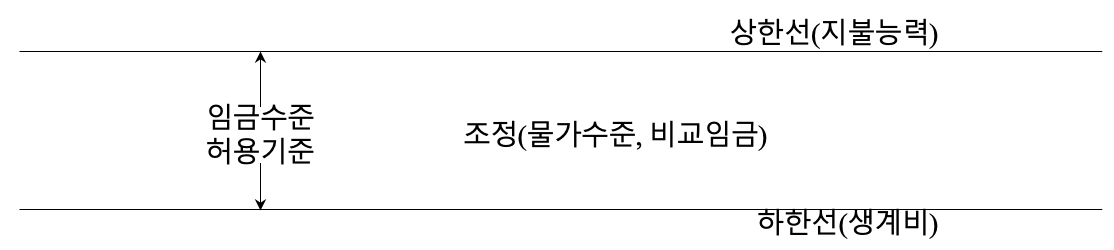
\includegraphics[width=.8\textwidth]{pic/임금수준}
        \caption{임금수준의 결정 모형}
    \end{figure}
\end{frame}

\begin{frame}[allowframebreaks]
    \frametitle{임금체계의 관리}
    \begin{block}{임금체계 (compensation structure)}
        피고용인에게 지급되는 임금이 어떠한 항목들로 구성되고 또한 각 임금항목이 어떠한 기준에 의해 결정되는가를 나타내 주는 개념
    \end{block}
    \begin{table}
        \centering
        \resizebox{.63\textwidth}{!}{\relax
                \begin{tabular}{cp{7cm}p{7cm}}
        \toprule
        & \textbf{장점} & \textbf{단점} \\
        \midrule
        \textbf{연공급} 
        & 생활보장으로 귀속의식 확대 \newline 연공질서 확립과 사기 유지 \newline 폐쇄적 노동시장에서 용이 \newline 실사가 용이 \newline 성과평가가 곤란한 직무에 적용 가능 
        & 동일노동에 대한 동일임금 실시간곤란 \newline 전문기술인력의 확보 곤란 \newline 능력있는 젊은 종업원의 사기 저하 \newline 인건비 부담 가중 \newline 소극적 근무태도 야기 \\
        \midrule
        \textbf{직무급} 
        & 능력주의 인사풍토 조성 \newline 인건비의 효율성 증대 \newline 개인별 임금차 불만 해소 \newline 동일노동에 대한 동일임금 실현 
        & 절차가 복잡 \newline 학력, 연공주의 풍토에서의 저항 \\
        \midrule
        \textbf{직능급} 
        & 능력주의 임금관리 실현 \newline 유용한 인재의 지속적 보유 \newline 종업원의 성장육구기회 제공 
        & 초과능력에 적용 곤란 \newline 직능평가가 어려움 \newline 적용 직종의 제한 \newline 직무 표준화가 선행되어야 함 \\
        \midrule
        \textbf{성과급 (개인성과급)} 
        & 생산성 향상, 종업원 소득 증대 \newline 감독의 필요성 감소 \newline 인건비 측정 용이 
        & 품질관련 문제 발생 가능성 \newline 종업원의 신기술 도입 저하 \newline 생산기계의 고장 시 종업원 불만 고조 \newline 작업장 내 인간관계 문제 발생 가능성 \\
        \bottomrule
    \end{tabular}

        }
        \caption{임금체계 비교}
    \end{table}
\end{frame}

\begin{frame}[allowframebreaks]
    \frametitle{회사의 임금정책}
    \begin{enumerate}[<+->]
        \item 선도전략 (lead strategy)
        \begin{itemize}[<+->]
            \item 경쟁기업의 일반적인 임금수준보다 높은 임금수준을 유지하는 전략
        \end{itemize}
        \item 동행전략 (match strategy)
        \begin{itemize}[<+->]
            \item 경쟁기업의 임금수준과 비슷한 수준을 유지하는 전략
        \end{itemize}
        \item 추종전략 (follow strategy)
        \begin{itemize}[<+->]
            \item 경쟁기업보다 낮은 임금수준을 유지하고 일정 기간의 격차를 두고 따라가는 전략
        \end{itemize}
    \end{enumerate}
\end{frame}

\begin{frame}[allowframebreaks]
    \frametitle{임금의 인접개념}
    \begin{enumerate}[<+->]
        \item 통상임금: 매월 정기적, 일률적, 고정적으로 지급되는 급여
        \begin{block}{통상임금 (근로기준법 시행령 제 6조 제 1항)}
            근로자에게 정기적으로, 일률적으로 (일정한 조건에 따른 모든 노동자에게), 고정적으로 (사전에 지급하기로 정해진) 소정근로 또는 총 근로에 대해 지급하기로 정한 시간급, 일급, 주급, 월급 금액 또는 도급 금액
        \end{block}
        \framebreak%
        \begin{itemize}[<+->]
            \item 종류: 책정된 기본급과 식대, 차량지원비, 통신지원금 등 매월 정기적으로 지급되는 급여
            \begin{itemize}[<+->]
                \item 직책수당, 위험작업수당, 자격증 수당 
                \item 정기상여금
            \end{itemize}
            \item 활용: 연장 야간 휴일 수당 산정, 연, 월차 수당 산정과 중도 퇴사자나 중도 입사자들의 근무일에 대한 급여 산정에 이용
            \item 산정 예: 12일치만 근무한 중도퇴사자의 급여는 1개월 통상임금을 30으로 나눈 금액이 1일 통상임금이므로 이 1일 통상임금에 12를 곱한 것이 12일치 급여가 됨
        \end{itemize}
        \framebreak%
        \item 평균임금: 정기적이든 부정기적이든 월급여로 받는 모든 금액
            \begin{itemize}[<+->]
                \item 종류: 통상임금과, 연월차수달, 야근수당, 추가근무수당 등 통상임금 외 각종 수당 등 월급여로 받는 모든 금액
                \item 산정기준: 평균임금 산정 사유 발생 직전 3개월의 금액을 기준으로 산정
                \item 활용: 퇴직금 산정에 이용.
                \item 예: 퇴직금 산정은 퇴직발령일 직전 3개월 간 받은 총 급여를 해당기간의 근무일수로 나눈 값이 `1일 평균임금'이 됨. 이 1일 평균임금에 30을 곱한 것이 1개월 평균임금이 되고 이 1개월 평균임금이 1년 근무에 대한 퇴직금이 됨
                \item 예: 산업재해보상금
            \end{itemize}
        \framebreak%
        \item 보수비용 (compensation costs)
            \begin{itemize}[<+->]
                \item 평균임금에 사용자부담금 (예: 의료보험, 산재보험 등 부담금)을 합한 금액
            \end{itemize}
        \item 노동비용 (labor costs)
            \begin{itemize}[<+->]
                \item 보수비용에 비용성 복리후생 (예: 출장비 등)과 인적자원에 대한 채용 및 교육비 등을 포함한 금액
            \end{itemize}
    \end{enumerate}
    \centering
    \begin{figure}
        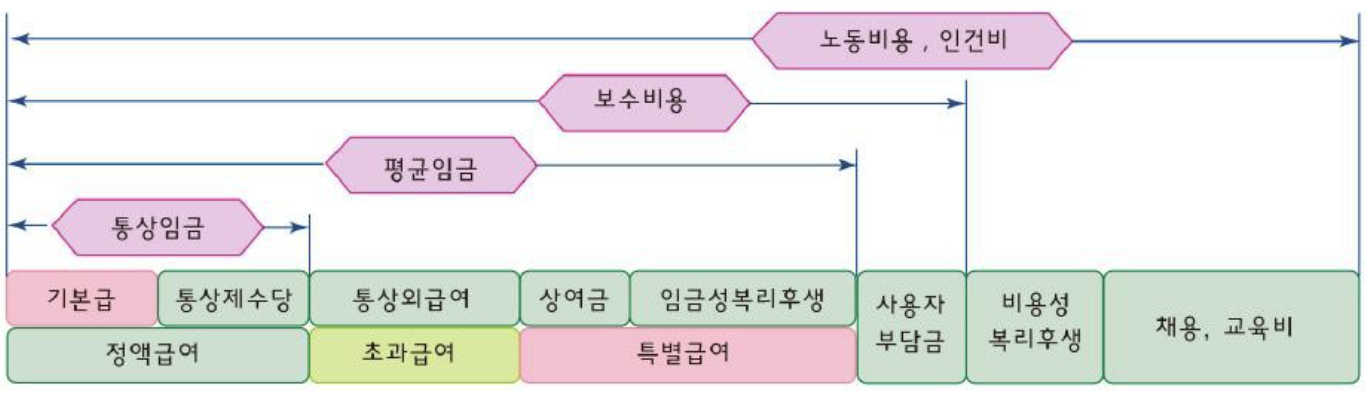
\includegraphics[width=.9\textwidth]{pic/임금범위.png}
        \caption{임금관련 제 개념의 명칭과 범위}
    \end{figure}
\end{frame}

\subsection{임금의 법적 보호제도}%

\begin{frame}
    \frametitle{근로기준법}
    \begin{itemize}[<+->]
        \item 가산급여: 연장근로, 야간근로, 휴일근로는 통상임금의 $\frac{50}{100}$ 이상을 가산하여 지급
        \item 도산·파산 시 임금지급: 사용자의 도산 또는 파산 시 임금채권의 우선변제 규정
        \begin{itemize}[<+->]
            \item 사용자가 도산 또는 파산하거나 사용자의 재산이 다른 채권자에 의하여 압류되었을 때, 피고용인의 임금채권을 일반채권자의 채권 또는 조세공과금보다 우선하여 변제 받도록 하는 동시에 피고용인의 최저생활보장을 확보하기 위한 사회정책적 제도
        \end{itemize}
        \item 휴업 시 임금지급: 사용자의 귀책사유로 인한 휴업의 경우 휴업기간 중 $\frac{70}{100}$ 이상의 수당을 지급하여야 함
        \begin{itemize}[<+->]
            \item 근로자의 생존권 확보를 목적으로 임금상실의 위험으로부터 근로자 보호
        \end{itemize}
    \end{itemize}
\end{frame}

\begin{frame}
    \frametitle{임금채권보장법}
    \begin{itemize}[<+->]
        \item 법의 목적: 경기의 변동 및 산업구조의 변화 등으로 사업의 계속이 불가능하거나 기업의 경영이 불안정하여 임금 등을 지급받지 못한 상태로 퇴직한 근로자에게 그 지급을 보장하는 조치를 강구함으로써 근로자의 생활안정에 이바지함
        \item 사업주가 파산한 경우 고용노동부 장관은 근로자의 청구가 있는 경우 근로자의 미지급 임금과 퇴직금을 임금채권보장기금으로 지급하고 그 지급한 금액의 한도 안에서 당해 사업주에 대한 당해 근로자의 미지급 임금 및 퇴직금 청구권을 대위
    \end{itemize}
\end{frame}

\begin{frame}[allowframebreaks]
    \frametitle{최저임금법}
    \begin{block}{최저임금제 (minimum wage system)}
        1894년 뉴질랜드에서 시작하여 현재 많은 선진국에서 도입하고 있는 제도로 국가가 노사간의 임금결정 과정에 개입하여 임금의 최하수준을 정하고 사용자에게 이 수준 이상의 임금을 지급하도록 법으로 강제하는 저임금 피고용인 보호제도
    \end{block}
    \begin{enumerate}[<+->]
        \item 의의: 국가가 임금의 최저수준을 결정하고 사용자에게 그 이상의 임금을 지급하도록 법률적으로 강제하는 제도
        \begin{itemize}[<+->]
            \item 국가의 기관이 조사•심의하여 결정한 최저의 임금 (법정최저금)을 법률적으로 강제하여 피고용인의 최저생계비를 보장해주는 제도
        \end{itemize}
        \framebreak%
        \item 목적: 사회•경제•산업정책적 목적
        \begin{itemize}[<+->]
            \item 사회정책적 목적: 저임금 피고용인 소득을 증대시켜 빈곤 퇴치, 교섭력이 미약한 미숙련•비조직 피고용인의 노동력 착취를 방지
            \item 경제정책적 목적: 저임금 피고용인의 구매력을 증대시켜 유효수요를 확대하고 불황에 발생하기 쉬운 임금절하로 인한 유효수요의 축소 방지
            \item 산업정책적 목적: 저임금에 의존하는 경쟁을 지양하고 기술개발 및 생산성 향상을 통한 기업간 공정 경쟁 유도 
        \end{itemize}
        \framebreak%
        \item 문제점·효과: 최저임금제의 도입에 따른 긍정적 측면과 부정적 측면 공존
        \begin{itemize}[<+->]
            \item 부정적 측면
            \begin{itemize}[<+->]
                \item 노동시장의 공급과잉 시 최저임금 이하의 성과를 창출하는 피고용인의 고용을 회피하여 실업률 증가 유발
                \item 최저임금은 인건비 인상을 초래하여 기업은 제품가격을 연쇄 인상하게 되어 그 부담은 결국 소비자에게 돌아가게 될 가능성이 있음
            \end{itemize}
            \item 국가 전체차원에서 최저생계비를 보장함으로써
            \begin{itemize}[<+->]
                \item 빈곤퇴치, 기업간 공정 경쟁유도
                \item 제품시장에서의 유효수요 창출
            \end{itemize}
            \item 최저임금제가 저임금 노동자에 미치는 영향
            \item 최저임금제가 영세자영업자, 중소 상공인 등에 미치는 영향
        \end{itemize}
        \item 최저임금 결정기구: 최저임금결정기구로 최저임금위원회 운영
        \begin{itemize}[<+->]
            \item 최저임금위원회 구성: 근로자위원, 사용자위원 및 공익위원 등 각 9명, 특별위원 3명,
            \item 임기: 3년 임기, 연임 가능
        \end{itemize}
    \end{enumerate}
\end{frame}

\subsection{우리나라의 임금현황}%

\begin{frame}[allowframebreaks]
    \frametitle{우리나라의 임금현황 개괄}
    \begin{itemize}[<+->]
        \item 임금성장률: 경제성장률 저하와 함께 임금성장률 역시 하락하는 추세.
        \item 성별: 여성 임금은 남성 임금수준에 비해 상대적으로 적지만 점차 개선되고 있음 (남성대비 66\%).
        \item 규모별: 대기업과 중소기업간의 임금격차는 심화되었음.
        \item 산업간 임금순위는 시대적으로 큰 변화는 보이지 않으나 산업간 임금격차는 많이 완화.
        \begin{itemize}[<+->]
            \item 금융·보험업 $>$ 전기·가스·수도업 등 장치산업 $> \cdots >$ 음식숙박업 $>$ 사업서비스업
        \end{itemize}
    \framebreak%
        \item 학력별: 한국의 임금체계는 학력중심의 임금구조가 강건했으나 최근 격차가 상당히 해소.
        \begin{itemize}[<+->]
            \item 저학력중심의 기능인력 부족 및 생산직 위주 노조활동에서 기인한 단체교섭의 결과.
        \end{itemize}
        \item 연령별: 45--49세를 정점으로 이후 하락.
        \begin{itemize}[<+->]
            \item 평균적으로 50대에 접어들면서 낮은 연봉의 직장으로 이직.
            \item 60세 정년의 실효성에 의문.
        \end{itemize}
    \end{itemize}
\end{frame}


\begin{frame}[allowframebreaks]
    \frametitle{임금체계와 결정방식}
    \begin{itemize}[<+->]
        \item 임금인상 결정방식: 노조와의 임금교섭. 노조가 없는 경우는 노사협의회를 통해
        \item 임금체계: 연공급적 성격이 강했으나 경제위기 후 연봉제, 성과배분제 등이 증가
        \begin{itemize}[<+->]
            \item 우리나라 기업의 임금체계: 주로 학력•성•근속 등 연공요소에 따라 직위 직급과 호봉을 산출하며 연공급적 성격이 강함
            \item 최근 연공서열 위주의 경직적인 임금체계를 연봉제•성과배분제 등 능력•성과위주 임금체계로 전환하려는 기업이 크게 증가 (단, 연공서열임금제도를 탈피한다는 것을 의미하지 않음)
        \end{itemize}
    \end{itemize}
\end{frame}

\subsection{임금제도의 최근 이슈}%

\begin{frame}[allowframebreaks]
    \frametitle{퇴직연금}
    \begin{block}{퇴직연금}
        기업이 퇴직금재원을 사내에 적립하던 퇴직금제도를 대체하여 금융기관에 매년 퇴직금 해당금액을 적립하여 근로자가 퇴직할 때 연금 또는 일시금으로 지급받아 노후설계가 가능하도록 하는 준 공적연금.
    \end{block}
    \begin{itemize}[<+->]
        \item 근로자퇴직급여보장법 
        \begin{itemize}[<+->]
            \item 2005년 12월부터 시행
            \item 2016년부터 300인 이상 기업 의무화, 2024년까지 전면 의무화됨. 
            \item 가입 후 10년 이상 유지해서 신청에 따라 만 5S세 이후부터 수령할 수 있음
        \end{itemize}
    \end{itemize}
    \framebreak%
    \begin{enumerate}[<+->]
        \item 도입배경: 고령화 및 저출산현상에 따른 노후대책 필요
        \begin{itemize}[<+->]
            \item 근로자: 퇴직금제도가 있었지만 중간정산으로 생활비로 소진
            \item 회사: 퇴직금 지급 재원을 별도로 적립하지 않고 기업 운영비로 활용하여 도산 시 퇴직금 체불 사례 빈번하게 발생
            \item 노후대책으로서 연금의 성격을 강화하고 기존 퇴직금제도의 수급불안을 해소하기 위해 도입
        \end{itemize}
    \framebreak%
        \item 종류
        \begin{itemize}[<+->]
            \item 확정급여형 (defined benefit: DB형): 최종 급여 액수가 사전에 정해짐, 급여액은 퇴직 전 평균임금에 연동, 회사가 부담하는 보험 기여금이 펀드 수익성에 따라 가변적일 수 있음
            \item 확정기여형 (defined contribution: DC형): 회사가 부담하는 기여금이 사전에 정해짐. 급여액은 펀드 운영성과에 의해 가변적임.
            \item 개인퇴직계좌 (individual retirement pension: IRP형): 잦은 이직이나 퇴직 등에 따른 적립 단절 문제에 대응, 재직자, 자영업자, 공무원 등 다른 연금 가입여부 상관없이 계좌를 만들 수 있음.
            \item 퇴직 연금은 중도인출을 엄격히 제한, 은퇴까지 적립 계좌를 유지함.
        \end{itemize}
    \framebreak%
        \item 장점과 단점
        \begin{itemize}[<+->]
            \item 장점
            \begin{itemize}[<+->]
                \item 기업도산에 따른 지급불능사태에 대응할 수 있음. $\because$ 외부 금융기관에 퇴직연금을 맡겨 놓아 사업장의 도산에도 떼일 염려가 없음
                \item 중간정산으로 노후재원을 마련하기 어려웠는데 중도인출 요건을 제한하여 노후생활자금 마련
            \end{itemize}
            \item 단점
            \begin{itemize}[<+->]
                \item 퇴직금 중간정산제 폐지
                \item 도입에서 노사간의 의견 불일치
                \item 은행이나 보험회사의 퇴직연금 설명으로 정보 왜곡
                \item 자본시장 활성화 목적
            \end{itemize}
        \end{itemize}
    \end{enumerate}
\end{frame}

\section{성과참가제도}%
\subsection{제도의 의의와 종류}%

\begin{frame}[allowframebreaks]
    \frametitle{제도의 의의}
    \begin{itemize}[<+->]
        \item 성과참가제도: 기업의 경영성과 달성에 직접•간접적으로 공헌한 이해관계자 집단간에 그 성과의 배분이 이루어지는 과정. 즉, 노사간의 협동적 노력을 통하여 증대되는 경영성과가 경영자나 자본가에게 독점되는 것이 아니라 그 중 일정한 부분을 기본급 이외의 참여적 임금으로 추가적으로 지급하는 제도
        \begin{itemize}[<+->]
            \item 피고용인에 대한 경제적 혜택 증대, 공동체의식 형성, 회사발전에 대한 자발적 노력 강화
        \end{itemize}
    \end{itemize}
\end{frame}

\begin{frame}[allowframebreaks]
    \frametitle{제도의 종류}
    \begin{itemize}[<+->]
        \item 종류: 성과배분기준 및 피고용인의 참여 여부에 따라 
        \begin{itemize}[<+->]
            \item 이익배분 (profit sharing): 정기적인 임금에 덧붙여 합리적인 적용원칙 하에 기업의 이윤을 기초로 모든 피고용인에게 지불하는 현금급부와 이연급부의 지급과정
            \item 성과배분 (gainsharing): 피고용인이 기업의 성과 향상을 위해 노력하여 발생한 이익을 금전적 형태로 피고용인에게 배분하는 제도 의사결정제도와 성과배분을 결합한 형태
        \end{itemize}
        \item 성공적인 성과배분제도: 효과적인 피고용인의 경영참가의 틀 및 보너스의 공평한 배분기준 확립 필요
    \end{itemize}
\end{frame}

\subsection{이익배분제도}%

\begin{frame}[allowframebreaks]
    \frametitle{제도의 유형}
    \begin{itemize}[<+->]
        \item 이연배분제도: 이윤배분 몫이 공제기금에 예치한 후 특정 사건 (예; 퇴직, 사망 등)이 발생하면 피고용인 계좌로 이체하는 제도
        \begin{itemize}[<+->]
            \item 공제기금은 자사 또는 타사 주식, 부동산 및 공채 등에 투자함
            \item 세제상의 혜택 부여, 연금 또는 퇴직금의 성격 (미국), 경영상의 신축성 확보 등의 장점
            \item 제도의 복잡성으로 관리나 설치에 상당한 어려움 존재
        \end{itemize}
    \framebreak%
        \item 현금배분제도: 현 시점에서의 이윤을 현금으로 일정한 배분기간 (예: 분기별)에 따라 배분 제도
        \begin{itemize}[<+->]
            \item 배분기간을 월별로 하면 정기적 임금으로 인식, 연간으로 하면 인센티브의 성격 약화. $\therefore$ 분기별이 바람직
        \end{itemize}
        \item 혼합배분제도: 현금배분제도와 이연배분제도의 절충형, 미래 급부에 현재의 추가적 보상 함유
        \begin{itemize}[<+->]
            \item 일정부분은 현금으로 배분하고 잔여분은 공제기금 형태로 지급
        \end{itemize}
    \end{itemize}
\end{frame}

\begin{frame}[allowframebreaks]
    \frametitle{제도의 효과}
    \begin{itemize}[<+->]
        \item 긍정적 효과
        \begin{itemize}[<+->]
            \item 기업측과 피고용인과의 협동정신 함양·강화 고용관계의 개선
            \item 피고용인은 자기의 이익 배당액을 증가시켜 작업에 열중 능률증진
            \item 피고용인의 이익배당 참가권과 분배율을 근속연수와 관련시켜 피고용인의 장기근속 장려
        \end{itemize}
        \item 부정적 측면 
        \begin{itemize}[<+->]
            \item 배당액의 변동 및 결산 후 배당이 이루어져 동기부여 효과 반감
            \item 회계상 이익으로 배당액수 결정: 기업 능력, 물가변동 등 외적 요인에 좌우, 회계 처리상 이익을 자의적으로 조정
            \item ∴ 이익배분 참가들의 동기유발 미흡
        \end{itemize}
        \item 실증연구 결과
        \begin{itemize}[<+->]
            \item 성과배분제도에 비하여 경영성과에 미치는 영향이 미약한 것으로 밝혀짐
            \item 단, 피고용인에게 노사가 공동운명체 임을 알리는 상징적 효과
        \end{itemize}
    \end{itemize}
\end{frame}

\subsection{참가형 성과배분제도}%

\begin{frame}[allowframebreaks]
    \frametitle{유형}
    \begin{itemize}[<+->]
        \item 참가형 성과배분은 집단보너스제도에 경영참가를 결합한 것으로 처음 미국에서 시작하여 현재 각국에서 실시
        \item 1930년대 Scanlon plan이 고안됨: 파산의 위기에 몰린 철강회사를 재건하는 데 주된 역할을 함
        \begin{itemize}[<+->]
            \item 노동비용을 생산액으로 나눈 비율을 사용하여 보너스 산정. 즉 과거의 실적에 따라 기준 비율을 정하고 이 비율보다 낮아졌을 때 절감한 노동비용을 노사가 배분하고 근로자에게 집단적으로 보너스 지급
        \end{itemize}
        \item 1940년대 Scanlon plan의 보너스 산정방식을 보다 안정된 계산방식으로 수정한 Rucker plan 등장
        \begin{itemize}[<+->]
            \item 노동비용을 부가가치로 나눈 비율을 보너스 산정공식으로 사용
        \end{itemize}
        \item 1970년대 Improshare 등장
        \begin{itemize}[<+->]
            \item 실제생산시간을 표준생산시간으로 나눈 비율을 보너스산정공식으로 사용: 산업공학의 원칙을 이용하여 보너스를 산정함
        \end{itemize}
        \item 최근에는 커스텀 플랜이 고안됨: 기존의 정형화된 프로그램을 각 기업의 환경과 상황에 맞추어서 수정하여 적용하는 참가형 성과배분제로 발전 
        \begin{itemize}[<+->]
            \item 성과측정의 기준으로 노동비용이나 생산비용, 생산성 뿐만 아니라 품질향상, 소비자 만족도 등을 새로운 지표로 사용
        \end{itemize}
    \end{itemize}
\end{frame}

\begin{frame}[allowframebreaks]
    \frametitle{성과}
    \begin{itemize}[<+->]
        \item 참가형 성과배분제도는 현장자율경영팀과 함께 경영참가제도 중 가장 긍정적 효과가 보임
        \begin{itemize}[<+->]
            \item ∵ 참가자의 참가욕구와 금전 욕구를 다 함께 만족시켜 동기유발효과가 크기 때문
        \end{itemize}
        \item 실증연구 결과 종합
        \begin{itemize}[<+->]
            \item 참가형 성과배분이 성공하는 비율은 50~80%이며, 평균 65% 기업이 긍정적 효과를 경험
            \item 생산성 향상에 가장 뚜렷한 효과를 보임
            \item 일부 연구에서는 참가형 성과배분제도가 제품품질향상에 긍정적 효과가 있는 것으로 나타남
            \item 참가형 성과배분제도가 고용관계 증진 효과, 종업원의 동기유발, 기업의 소속감 향상에 효과가 있음
        \end{itemize}
        \item 우리나라 성과참가제도
        \begin{itemize}[<+->]
            \item 참여형 성과배분제도를 실사하는 경우가 적고, 이익배분제도를 실시하는 경우가 상대적으로 많음
        \end{itemize}
    \end{itemize}
\end{frame}

\section{자본참가제도}%

\begin{frame}[allowframebreaks]
    \frametitle{제도의 개념}
    \begin{itemize}[<+->]
        \item 자본참가: 피고용인으로 하여금 자본의 출자자로서 기업경영에 참가시키고자 하는 것으로 소유참가, 재산참가라고도 함
        \item 자본참가의 형태: 우리사주제도 및 스톡옵션 (Stock Option)제도 등이 있음
        \begin{itemize}[<+->]
            \item 스톡옵션제도는 최근 벤처기업에서 피고용인의 동기유발기법으로 각광 받고 있음
        \end{itemize}
    \end{itemize}
\end{frame}

\subsection{우리사주제도}%
\begin{frame}[allowframebreaks]
    \frametitle{특징}
\begin{block}{우리사주제도 (Employee Stock Ownership plan; ESOPs)}
    자본참가의 대표적인 유형으로서 고용관계의 대책으로서 또는 안정주주의 확보라는 기업 방어적인 관점 및 피고용인의 재산형성 촉진의 일환으로 장려
    \end{block}
    \begin{itemize}[<+->]
        \item 회사의 경영방침으로서 피고용인에게 자사 주식을 보유하도록 추진 
        \begin{itemize}[<+->]
            \item ∴ 피고용인이 독자적으로 자기의사에 의해 자사주를 구입한 경우는 해당되지 않음.
        \end{itemize}
        \item 회사의 특별한 편의 제공: 
        \begin{itemize}[<+->]
            \item 자금의 보조: 장려금의 교부 및 매매수수료의 부담
            \item 매입자금의 대부: 구입자본의 무이자 또는 저리대부, 구입자금의 분할변제, 자금융자의 알선, 주식의 저가 양도 또는 공로주의 증여 등
        \end{itemize}
        \item 자사주의 취득 및 장기보유: 피고용인의 재산형성정책인 동시에 회사의 주식안정정책
        \item 자사주의 취득•보유가 제도화 되려면 증자 시에 자사주 구입운동같은 것이 아닌, `자사주 투자회'와 같이 항구적이어야
    \end{itemize}
\end{frame}

\begin{frame}[allowframebreaks]
    \frametitle{중요성}
    \begin{itemize}[<+->]
        \item 고용관계적 중요성
        \begin{itemize}[<+->]
            \item 피고용인에게 주주의 지위 부여 $\implies$ 피고용인이 경영과 분배 참여 $\implies$ 노사협조 촉진
            \item 회사의 경영이 피고용인 자신의 이익과 직결 $\implies$ 근로의욕 고취, 생산성 향상 및 애사정신 함양
            \item 피고용인에게 재산형성의 기회 제공 $\implies$ 노동력의 정착성 증진
        \end{itemize}
        \item 재무관리적 중요성: 자본조달의 수단으로 활용할 수 있으며 주주의 안정성 도모 및 주가안정 $\implies$ 기업지배의 방지효과
        \item 상장법인의 결성률이 코스닥법인 결성률보다 높음 $\implies$ 우리사주제도 실시는 매출규모나 영업이익 규모 등과 긍정적인 상관관계를 보임
    \end{itemize}
\end{frame}

\subsection{스톡옵션제도}%

\begin{frame}[allowframebreaks]
    \frametitle{도입배경}
    \begin{block}{스톡옵션 (Stock Option)제도} 
        회사가 임•직원에게 일정기간 내에 자기회사의 주식을 사전에 약정된 가격으로 일정 수량만큼 매수할 수 있는 권리를 부여하는 제도로 `주식매입선택권' 이라고도 함
    \end{block}
    \begin{itemize}[<+->]
        \item 도입 취지: 경제활성화를 위한 국민경제의 기반을 이루는 벤처기업 등에 유능한 인재 유치 구축
        \item ∵ 중소창업기업의 경우 유동성이 적어서 어려움을 겪을 가능성이 많기 때문에 고급인력의 확보 및 유지를 위해 스톡옵션제도를 활용하면 많은 문제점이 해소될 수 있음
    \end{itemize}
\end{frame}

\begin{frame}[allowframebreaks]
    \frametitle{도입현황}
    \begin{itemize}[<+->]
        \item 스톡옵션제도를 실시하는 기업이 조사대상기업의 약 5\% 내외
        \begin{itemize}[<+->]
            \item 규모: 기업규모가 클수록
            \item 업종: 금융보험 및 부동산업
            \item 소유형태: 독립 전문경영체제를 가진 기업
            \item 고용관계 성격: 협력적 고용관계
        \end{itemize}
    \end{itemize}
\end{frame}



%------------------------------------------------
\end{document}
%------------------------------------------------

